\chapter{Requirements}

\section{Use cases}

As with all requirements specifications, a good place to begin was to create various use case diagrams representing the roles in the system and the actions they ought to be able to perform. By doing so, it would also be possible to derive common classes and actions by examining similar or duplicating use case scenarios.

\subsection{Registration}

\begin{figure}[h!]
  \centering
    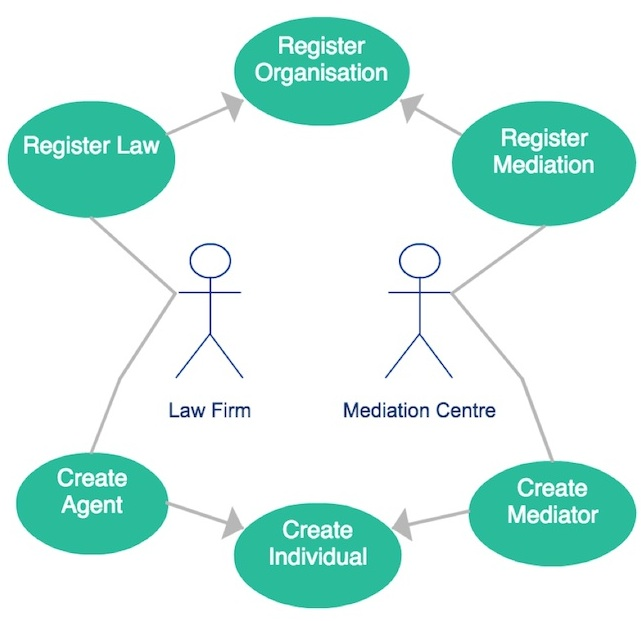
\includegraphics[width=\textwidth]{use_case--registration}
  \caption{Use case diagram showing registration feature}
  \label{uml:useCase:registration}
\end{figure}

Authorised individuals should be allowed to register accounts representing their company (be it a law firm or mediation centre), and that within that organised account they should be able to register individual accounts, which should be agents or mediators depending on the organisation type.

Figure ~\ref{uml:useCase:registration} shows this in terms of the law firms and mediation centres. In both the organisational and individual registration, a generalised action has been added which these more specific actions can extend or implement, showing where it might be possible to use a common class or database table to accomplish both goals.

\subsection{Disputes}

\begin{figure}[h!]
  \centering
    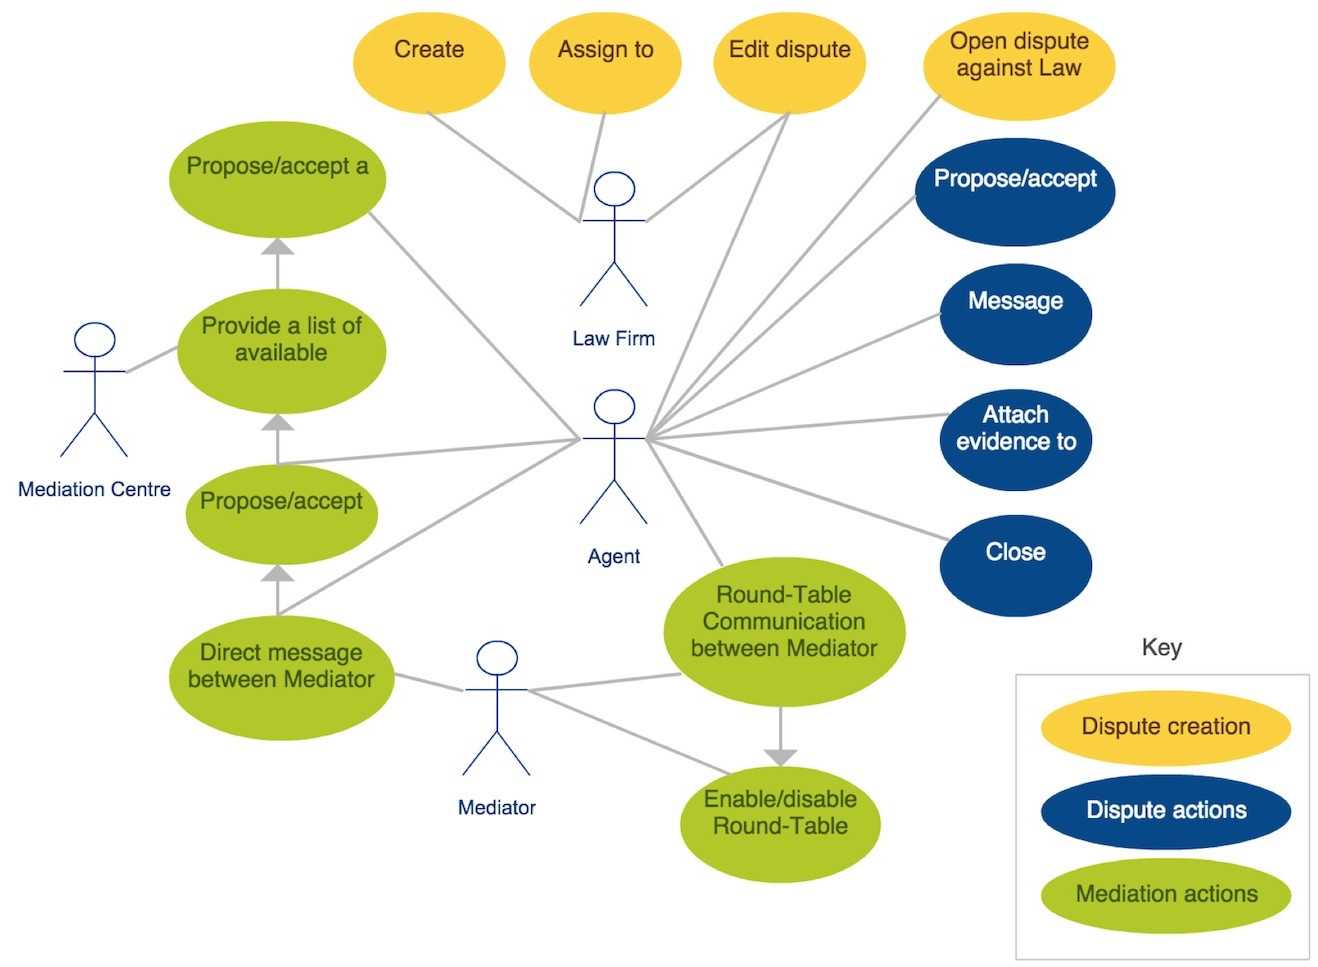
\includegraphics[width=\textwidth]{use_case--disputes}
  \caption{Use case diagram showing actions available in a dispute}
  \label{uml:useCase:disputes}
\end{figure}

Figure~\ref{uml:useCase:disputes} shows the roles and actions involved in the creation, mediation and closing of a dispute.

Only law firms can create new disputes. There is then some back-and-forth assignment between law firms and agents until both sides of a dispute are represented by different agents. This is identified as being the ``dispute creation" stage.

Inside a dispute, agents should be able to negotiate the dispute lifespan, exchange messages and evidence, and should have the freedom to close a dispute. In a best-case scenario, this is all that is required to successfully resolve a dispute. This is known as the ``dispute" stage.

Should it be required, an agent can propose mediation, and there is a defined process of administration between the agents and mediation centre required to get the dispute `in mediation'. Once in this state, the agents can communicate only through the mediator, unless the mediator feels the dispute is close to resolution and decides to enable round-table communication.

\subsection{Miscellaneous}

\begin{figure}[h!]
  \centering
    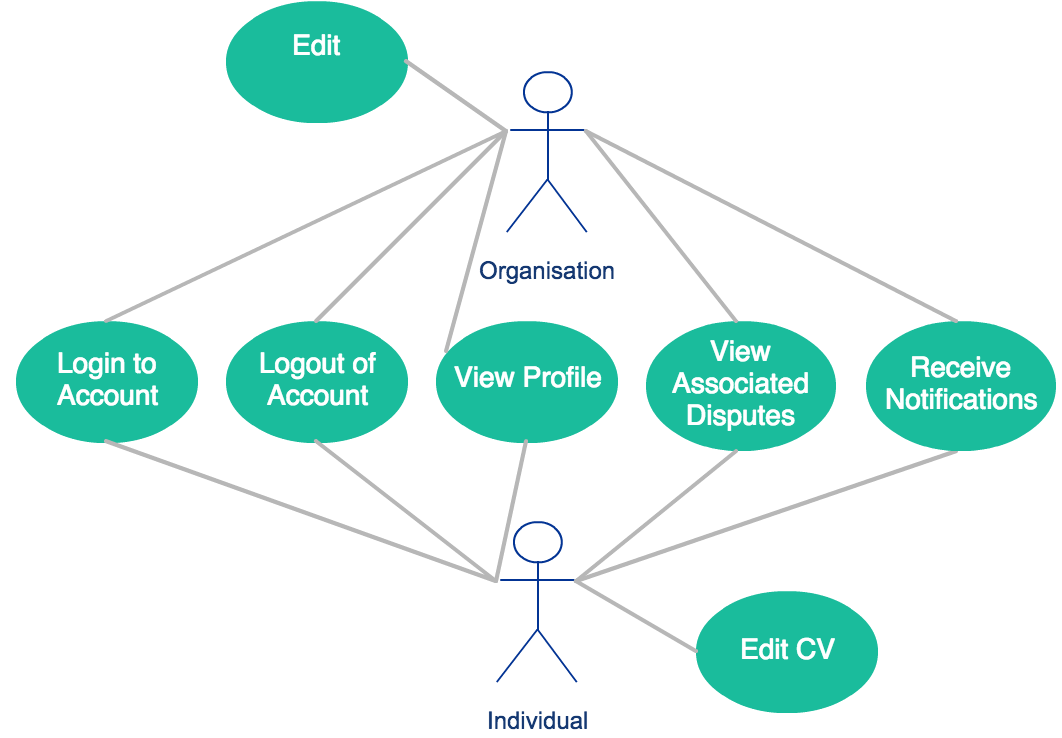
\includegraphics[width=\textwidth]{use_case--miscellaneous}
  \caption{Use case diagram demonstrating other miscellaneous requirements}
  \label{uml:useCase:miscellaneous}
\end{figure}

Other, lesser elements of functionality are shown by the miscellaneous UML diagram in figure~\ref{uml:useCase:miscellaneous}. For example, agents should be able to peruse a mediator's CV before making a decision as to which mediator to opt for. This suggests a ``view profile" facility, with custom fields for the CV, which could be as simple as a HTML textarea or as complicated as an integrated PDF uploader and viewer.

Given the tight deadline of the project and the scale of the system, coupled with the high priority of demonstrating some maritime collision logic, it was decided that these miscellaneous features should be kept as simple as possible.

\section{Features}

Following on from the use case diagrams, it was critical to explicitly define the project requirements in some textual way. Given that the project will embody agile principles, it makes sense to document these features in a testable way.

@TODO - discuss language choices etc before this point. Move it from the design to the requirements.

Business-driven development (BDD) allows you to mark up features in a human-readable way, so that a business analyst is able to understand the requirements but does not need to know the technical implementation. However, the features do follow a convention (the Gherkin syntax - [REF]), where each feature step has a corresponding step definition represented in code. This makes the features executable and allows automated end-to-end testing.

The PHP de-facto standard implementation of BDD is Behat, but through heavy discussion on which BDD framework to use (see appendix~\ref{appendix:bdd}), it was decided that the project should use Ruby and Cucumber.

Appendix ~\ref{appendix:requirements} contains the full set of Cucumber features, which form the basis of the requirements specification.